%\section{Specific Flooding and Routing Protocols for Wireless Multi-Hop Ad hoc Networks}
\section{IETF Routing Protocols for Spontaneous Wireless Networks}
\label{s:specific}
%
Since the late 1990s, in parallel with the emergence and deployment of new and more flexible networking technologies, the IETF has embarked upon a path of designing, developing and standardizing new routing protocols and flooding mechanisms. These protocols and mechanisms are designed for networks with increasingly more fragile and low-capacity links, with less pre-determined connectivity properties and with increasingly constrained router resources. \ \\ \ \\
%
Most of the IETF protocol design and standardization activity has focused on protocols designed for Mobile Ad hoc Networks (MANETs) and Low-Power Lossy Networks (LLNs), both defined in section \ref{ss:manet_lln}. This section presents the main flooding and routing protocols designed and standardized by the IETF for these types of networks in the last years: OLSRv1 and OLSRv2, RPL, AODV and LOADng.
%
\paragraph{Routing in MANETs: OLSR and AODV}
%
IETF activities targeting MANETs have converged on the development of two protocols, each one representative of one of the two main routing families (see section \ref{ss:routing}): reactive and proactive routing. \ \\ \ \\
%
IETF design and standardization work in the reactive routing realm for mobile ad hoc networks first led to the Ad-hoc On-demand Distance Vector protocol (AODV) \cite{rfc3561}; the efforts in proactive routing, in turn, led to the Optimized Link State Routing (OLSR) \cite{rfc3626}. A distance vector protocol, AODV operates in an \textit{on-demand} fashion, acquiring and maintaining routes only while needed for carrying data, by way of \textit{Route Request}-\textit{Route Reply} exchanges. A link state protocol, OLSR is based on periodic control messages exchanges, and each router proactively maintaining a routing table with entries for all destinations in the network. OLSR provides low delays in forwarding and has a predictable, constant control overhead -- at the expense of requiring memory in each router for maintaining complete network topology. AODV limits the memory required for routing state to that for actively used routes -- at the expense of delays for the \textit{Route Request}-\textit{Route Reply} exchange to take place, and control overhead dependent on data flows. \ \\ \ \\
%
Based on the operational experience acquired through AODV and OLSRv1, the IETF is currently designing and developing successors for OLSR and AODV. In the first case, the IETF community involved in OLSR has standardized OLSR version 2 (OLSRv2) \cite{OLSRv2} and its related components (packet format \cite{rfc5444} \cite{rfc5497}, NHDP \cite{rfc6130}). Work on AODV version 2 \cite{ietf:aodvv2} has started, as AODV derivative flourished: IEEE 802.11s \cite{IEEE-802.11s-principles}, which is based on AODV, and the G3-PLC standard \cite{itu:PLC-G3}, published in 2011, which specifies the use of the {\em 6LoWPAN Ad hoc Routing Protocol} (LOAD, specified in {\tt draft-daniel-6lowpan-adhoc-routing}) \cite{ietf:I-D:LOAD} at the MAC layer, for providing layer 2 routing for utility (electricity) metering networks. 
%
\paragraph{Routing in LLNs: RPL and LOADng}
%
LLNs can be regarded as a subset of MANETs, but with more stringent constraints in terms of device CPU and memory limitations, and work over more fragile links. Concerning LLNs, two protocols can be highlighted: RPL and LOADng. The IETF explored the problems of routing and adaptation of IPv6 for operation over the IEEE 802.15.4 MAC protocol, accommodating characteristics of that MAC layer, and with a careful eye on resource constrained devices (memory, CPU, energy, ...). Two initial approaches to such routing were explored: {\em mesh-under} and {\em route-over}. Both approaches entail different additional assumptions on the (link) characteristics of the addressed spontaneous wireless network, not present in the general networking model described in section \ref{ss:model}.
	\begin{enumerate}
	\item The {\em mesh-under} approach performs L2.5 multi-hop routing, that is, provides routing in an adaptation layer between 802.15.4 (MAC layer, L2) and IP (network layer, L3). This L2.5 routing enables the underlying mesh-routed multi-hop topology to be presented at the network layer as a single broadcast domain.
	\item The {\em route-over} approach, in contrast, exposes the underlying multi-hop topology to the IP layer, whereupon IP routing would build multi-hop connectivity. 
	\end{enumerate}
The IETF efforts on routing over 802.15.4 initially led to LOAD \cite{ietf:I-D:LOAD}, a derivative of AODV adapted for L2-addresses and mesh-under routing, and with some simplifications over AODV (\eg~removal of intermediate node replies and sequence numbers). However, 6LoWPAN was addressing other issues regarding adapting IPv6 for IEEE 802.15.4, such as IP packet header compression, and efforts to solve routing issues were suspended. In parallel with these efforts, the IETF has also specified the ``Routing Protocol for Low-power lossy networks'' (RPL), designed to support 6LoWPAN networks in a route-over configuration \cite{rfc6550, rpl-ipso}. \ \\ \ \\
%
However, reasons for using a simplified reactive approach instead of RPL have emerged, including better support for bi-directional data flows such as a request/reply of a meter reading \cite{RPL-bidirectional}, as well as algorithmic and code complexity reasons \cite{RPL-criticism}. These observations led on one hand to a renewed interest in AODV-derived protocols for specific scenarios, resulting in LOADng \cite{ietf:I-D:LOADng} \cite{ietf:I-D:LOADng-interop} and AODVv2 \cite{ietf:aodvv2}, while on the other hand leading to the development of an extension of RPL to support reactive path discovery (P2P-RPL \cite{ietf:rpl-p2p}).
%
% However, 6LowPAN was addressing other issues regarding adapting IPv6 for IEEE 802.15.4, such as IP packet header compression, and solving the routing issues was suspended, delegated to a working group ROLL, created in 2008 for this purpose. ROLL produced a routing protocol denoted ``Routing Protocol for Low-power lossy networks'' (RPL)  \cite{ietf:RFC6550:RPL} in 2012.
%
%Part of the original charter for this working group was to develop protocols for routing in multi-hop topologies under such constrained conditions, and over this particular MAC. Two initial philosophies to such routing were explored: {\em mesh-under} and {\em route-over}. The former, mesh-under, would, as part of an adaptation layer between 802.15.4 and IP, provide L2.5 multi-hop routing, presenting an underlying mesh-routed multi-hop topology as a single IP link. The latter, route-over, would expose the underlying multi-hop topology to the IP layer, whereupon IP routing would build multi-hop connectivity. Several proposals for routing were presented in 6LowPAN, for each of these philosophies, including LOAD \cite{ietf:I-D:LOAD}. LOAD was a derivative of AODV, but adapted for L2-addresses and mesh-under routing, and with some simplifications over AODV (\eg~removal of intermediate node replies and sequence numbers). However, 6LowPAN was addressing other issues regarding adapting IPv6 for IEEE 802.15.4, such as IP packet header compression, and solving the routing issues was suspended, delegated to a working group ROLL, created in 2008 for this purpose. ROLL produced a routing protocol denoted ``Routing Protocol for Low-power lossy networks'' (RPL) \cite{ietf:RFC6550:RPL} in 2012.
%
%Justifications for using an AODV derivative in preference to RPL include that the former better supports bi-directional data flows such as a request/reply of a meter reading \cite{RPL-bidirectional}, as well as algorithmic and code complexity reasons \cite{RPL-criticism}. The emergence of LLNs thus triggered a renewed interest in AODV-derived protocols for specific scenarios, resulting in work within the IETF \cite{ietf:I-D:LOADng} and \cite{ietf:I-D:LOADng-interop} for the purpose of standardization of  LOADng, incorporating the experiences from deploying AODV -- including, but not only, in LLNs.
%
%Since the late 1990s, the IETF has embarked upon a path of developing routing protocols for networks with increasingly more fragile and low-capacity links, with less pre-determined connectivity properties and with increasingly constrained router resources. In '97, by chartering the MANET working group, then subsequently in 2006 and 2008 by chartering the 6LowPAN and ROLL working groups.
%
%\paragraph{MANET Protocol Developments}
%The MANET working group converged on the development of two protocol families: reactive protocols, including AODV  \cite{AODV-RFC3561}, and proactive protocols, including  Optimized Link State Routing (OLSR) \cite{OLSR-RFC3626}.  A distance vector protocol, AODV operates in an \textit{on-demand} fashion, acquiring and maintaining routes only while needed for carrying data, by way of a \textit{Route Request}-\textit{Route Reply} exchange. A link state protocol, OLSR is based on periodic control messages exchanges, and each router proactively maintaining a routing table with entries for all destinations in the network, which provides low delays but constant control overhead.  A sizable body of work exists, including \cite{SIMCOMP}, studying the performance of these protocols in different scenarios, and justifying their complementarity \cite{LIX-NET-journal-1}.  OLSR provides low delays and predictable, constant control overhead -- at expense of requiring memory in each router for maintaining complete network topology. AODV limits the memory required for routing state to that for actively used routes -- at the expense of delays for the \textit{Route Request}-\textit{Route Reply} exchange to take place, and control overhead dependent on data flows.
%
%After acquiring operational experiences, the MANET working group commenced developing successors to OLSR and AODV, denoted OLSRv2 and DYMO. Whereas a relatively large and active community around OLSR thus standardized OLSRv2 \cite{jitter-RFC5148}, \cite{packetbb-RFC5444}, \cite{tlv-RFC5497}, \cite{NHDP-RFC6130} and \cite{OLSRv2}, the momentum behind DYMO withered in the MANET working group\footnote{http://tools.ietf.org/wg/manet/minutes?item=minutes81.html}.
%
%In the meantime, AODV derivative live on: IEEE 802.11s \cite{IEEE-802.11s-principles} is based on AODV, and the G3-PLC standard  \cite{itu:PLC-G3}, published in 2011, specifies the use of \cite{ietf:I-D:LOAD} at the MAC layer, for providing mesh-under routing for utility (electricity) metering networks. Justifications for using an AODV derivative in preference to RPL include that the former better supports bi-directional data flows such as a request/reply of a meter reading \cite{RPL-bidirectional}, as well as algorithmic and code complexity reasons \cite{RPL-criticism}. The emergence of LLNs thus triggered a renewed interest in AODV-derived protocols for specific scenarios, resulting in work within the IETF \cite{ietf:I-D:LOADng} and \cite{ietf:I-D:LOADng-interop} for the purpose of standardization of  LOADng, incorporating the experiences from deploying AODV -- including, but not only, in LLNs.
%
%\paragraph{6LowPAN and ROLL Protocol Developments}
%
%The 6LowPAN working group was chartered for adapting IPv6 for operation over IEEE 802.15.4, accommodating characteristics of that MAC layer, and with a careful eye on resource constrained devices (memory, CPU, energy, ...). Part of the original charter for this working group was to develop protocols for routing in multi-hop topologies under such constrained conditions, and over this particular MAC. Two initial philosophies to such routing were explored: {\em mesh-under} and {\em route-over}. The former, mesh-under, would, as part of an adaptation layer between 802.15.4 and IP, provide L2.5 multi-hop routing, presenting an underlying mesh-routed multi-hop topology as a single IP link. The latter, route-over, would expose the underlying multi-hop topology to the IP layer, whereupon IP routing would build multi-hop connectivity. Several proposals for routing were presented in 6LowPAN, for each of these philosophies, including LOAD \cite{ietf:I-D:LOAD}. LOAD was a derivative of AODV, but adapted for L2-addresses and mesh-under routing, and with some simplifications over AODV (\eg~removal of intermediate node replies and sequence numbers). However, 6LowPAN was addressing other issues regarding adapting IPv6 for IEEE 802.15.4, such as IP packet header compression, and solving the routing issues was suspended, delegated to a working group ROLL, created in 2008 for this purpose. ROLL produced a routing protocol denoted ``Routing Protocol for Low-power lossy networks'' (RPL)  \cite{ietf:RFC6550:RPL} in 2012.
%
\subsection{Optimized Link State Routing Protocol (OLSR)}
\label{sec:olsr}
%
OLSR is developed for mobile ad hoc networks, and operates as a  table driven, proactive protocol, i.e., it exchanges topology information with other routers in the network regularly. The key concept used in the protocol is that of multipoint relays (MPRs, described in section \ref{ss:flood}), selected nodes which forward broadcast messages during the flooding process. This efficient flooding technique substantially reduces the message overhead as compared to a classical flooding mechanism. \ \\ \ \\
%
OLSR version 1 was standardized in RFC 3626 \cite{rfc3626}. The work continues as OLSR version 2 (OLSRv2 \cite{OLSRv2}), which retains the same basic algorithms as its predecessor, however offers various improvements, {\em e.g.} a modular and flexible architecture allowing extensions, such as security, to be developed as add-ons to the basic protocol. \ \\ \ \\
%
%(new)
Every router running OLSR in the network generates two types of messages: {\em Hellos} and {\em Topology Control} (TC) messages. Information collected through exchange of these messages allows routers to perform the three basic processes of OLSR: Neighborhood Discovery, Link State Advertisements and Routing Set Calculation. Because OLSR (version 1) and OLSRv2 shares the same basic mechanisms, the text below applies to both protocols. 
%
%\paragraph{Routing Control Messages}\label{sec:olsr-msg}
%
%Every router running OLSR in the network generates two types of messages: Hellos and TC (Topology Control), to exchange topology information of the network. 
%
%\begin{itemize}
%\item {\bf Hello messages}. Hello messages are exchanged between a router and its 1-hop neighbors for neighbor discovery purposes, as explained in section \ref{ss:nd}. They can be generated proactively at a regular interval or as a response to a change in the router itself. In OLSR, a Hello message contains the local interface address(es), and its 1-hop neighbor addresses. With the broadcast of Hello messages to the router's 1-hop neighbor, the router is able to get the topology information in two hops. 
%\item {\bf Topology Control (TC) messages}. TC messages are broadcast by each node to the whole network to build the intra-forwarding database needed for routing packets. A TC message is sent by a node in the network to declare a set of links, which must include at least the links to all nodes of its MPR Selector set, {\em i.e.}, the neighbors which have selected the sender node as a MPR. TC messages are flooded to all nodes in the network and take advantage of MPRs. MPRs enable a better scalability in the distribution of topology information. With the broadcast of TC messages to the whole network, the node is able to get the topology information that is more than two hops away.
%\end{itemize}
%
\paragraph{Neighborhood Discovery}
%
OLSR routers discover their neighborhood by exchanging Hello messages with their 1-hop neighbors, as explained in section \ref{ss:nd}. These Hello messages can be generated proactively at a regular interval or as a response to a change in the router itself. In OLSR, a Hello message contains the local interface address(es), and its 1-hop neighbor addresses. With the broadcast of Hello messages to the router's 1-hop neighbor, the router is able to get the topology information in two hops.
%
%Hello messages are exchanged between a router and its 1-hop neighbors for neighbor discovery purposes, as explained in section \ref{ss:nd}. They can be generated proactively at a regular interval or as a response to a change in the router itself. In OLSR, a Hello message contains the local interface address(es), and its 1-hop neighbor addresses. With the broadcast of Hello messages to the router's 1-hop neighbor, the router is able to get the topology information in two hops.
%
\paragraph{Link State Advertisements}
%
%TC messages are broadcast by each node to the whole network to build the intra-forwarding database needed for routing packets. A TC message is sent by a node in the network to declare a set of links, which must include at least the links to all nodes of its MPR Selector set, {\em i.e.}, the neighbors which have selected the sender node as a MPR. TC messages are flooded to all nodes in the network and take advantage of MPRs. MPRs enable a better scalability in the distribution of topology information. With the broadcast of TC messages to the whole network, the node is able to get the topology information that is more than two hops away.
%
Link State Advertisement is the process where by the determined link state information is advertised through the network. For OLSR, this process is optimized by MPR flooding. MPR selection is encoded in outgoing Hellos. \ \\ \ \\
%
% JACF: Jiazi, I replaced the "planned" term for "managed", with a small explanation (as requested by reviewers). Is the notion correct?
Routers may express, in their Hello messages, their ``willingness'' (integer between 1 ``will never'' and 7 ``will always'') to be selected as MPR, which is taken into consideration for the MPR calculation. This is useful, for example, when an OLSRv2 network is {\em managed}, meaning that its topology is known or predictable. The set of routers having selected a given router as MPR is the MPR-selector-set of that router.  Each router must advertise, at least, all links between itself and its MPR-selector-set, in order to allow all routers to calculate shortest paths. \ \\ \ \\
%
Such link state advertisements are carried in Topology Control (TC) messages. TC messages are broadcast by each node to the whole network to build the intra-forwarding database needed for routing packets. A TC message is sent by a node in the network to declare a set of links, which must include at least the links to all nodes of its MPR Selector set, {\em i.e.}, the neighbors which have selected the sender node as a MPR. TC messages are received by all nodes in the network, by way of the MPR flooding process described above. With the broadcast of TC messages to the whole network, the node is able to get the topology information that is more than two hops away. TCs are sent periodically, however certain events may trigger non-periodic TCs.
%
%MPRs enable a better scalability in the distribution of topology information.
%
% broadcast through the network using the MPR flooding process described above. As a router selects MPRs only from among bi-directional neighbors, links advertised in TC are also bi-directional and routing paths calculated by OLSRv2 contain only bi-directional links. 
%
%Each router must advertise, at least, all links between itself and its MPR-selector-set, in order to allow all routers to calculate shortest paths. Such link state advertisements are carried in Topology Control (TC) messages, broadcast through the network using the MPR flooding process described above. As a router selects MPRs only from among bi-directional neighbors, links advertised in TC are also bi-directional and routing paths calculated by OLSRv2 contain only bi-directional links. TCs are sent periodically, however certain events may trigger non-periodic TCs.
%
\paragraph{Routing Set Calculation}
%
The Routing Set of a router is populated with Routing Tuples that represent paths from that router to all destinations in the network.  These paths are calculated based on the Network Topology Graph, which is constructed from information in the Information Bases, obtained via Hello and TC message exchange. \ \\ \ \\
%
Changes to the Routing Set do not require any messages to be transmitted.  The state of the Routing Set should, however, be  reflected in the IP routing table by adding and removing entries from that routing table as appropriate.  Only appropriate Routing Tuples  (in particular only those that represent local links or paths to routable addresses) need to be reflected in the IP routing table. \ \\ \ \\
%
OLSR does not mandate which algorithm to be used for path calculation, as along as the shortest paths for all destinations from all local OLSR interfaces can be obtained using Network Topology Graph. One example is Dijkstra's algorithm \cite{dijkstra59}. 
%
\subsection{Ad Hoc On-Demand Distance-Vector Protocol (AODV)}
\label{ss:aodv}
%
The Ad hoc On-Demand Distance Vector (AODV) \cite{rfc3561} protocol enables dynamic, self-starting, multi-hop routing between participating mobile  routers wishing to establish and maintain an ad hoc network.  AODV allows mobile nodes to obtain routes quickly for new destinations,  and does not require nodes to maintain routes to destinations that  are not in active communication. \ \\ \ \\
%
Compared to pro-active protocols like OLSR, AODV is more suitable under following constraints:
%
\begin{itemize}
\item Few concurrent traffic flows in the network (i.e., traffic flows only between few sources and destinations);
\item Little data traffic overall, and therefore the traffic load from periodic signaling (for proactive protocols) is greater than the  traffic load from flooding RREQs (for reactive protocols);
\item State requirements on the router are very stringent, i.e., it is beneficial to store only few routes on a router.
\end{itemize}
%
AODV was initially standardized as an experimental RFC in 2003 \cite{rfc3561}. Derivatives of AODV include 802.11s (with HWMP \cite{IEEE-802.11s-principles}) and LOADng \cite{ietf:I-D:LOADng}. In the following of this section, the basic mechanisms of AODV, \textit{Route Discovery} and \textit{Route Maintenance} are explained. Then a main derivative work of AODV, called LOADng, is also introduced. Note that at the time of writing, work on AODVv2 \cite{ietf:aodvv2} has just started, and thus we will not elaborate further on AODVv2 in this chapter.
%
\paragraph{Route Discovery}
%
The route discovery process is initiated when a source router needs a route to a destination router and it does not have a route in its routing table. The source router floods the network with a RREQ packet specifying the destination for which the route is requested. When the destination router, or an intermediate router with sufficiently up-to-date information about the requested destination, receive the RREQ packet, they generate a Route Reply (RREP) packet, which is sent back to the source along the reverse path. Each router along the reverse path sets up a forward pointer to the router it received the RREP from. This sets up a forward path from the source to the destination.
%
\paragraph{Route Maintenance}
%
When a router detects a broken link while attempting to forward a packet to the next hop, it generates a RERR packet that is sent to all sources using the broken link. The RERR packet erases all routes using the link along the way. If a source receives a RERR packet and a route to the destination is still required, it initiates a new route discovery process.
%
\subsubsection{Lightweight On-demand Ad hoc Distance-Vector (LOADng)}
%\subsubsection{Lightweight On-demand Ad hoc Distance-Vector Protocol (LOADng)}
%
The {\em Lightweight On-demand Ad hoc Distance-vector Routing Protocol - Next Generation} (LOADng) \cite{ietf:I-D:LOADng} is derived from AODV. Compared to AODV \cite{rfc3561}, it has more concise and flexible message format, and simplified message processing, which makes it more adapted to networks with constrained devices, such as sensor networks. It is also used for ITU Standard G. 9956 \cite{itu:PLC-G3}. \ \\ \ \\
%
Compared to AODV, LOADng has both simplifications and extensions to be more suitable to LLNs:
%
\begin{itemize}
\item Only the destination is permitted to respond to an RREQ;  intermediate LOADng Routers are explicitly prohibited from responding to RREQs, even if they may have active routes to the  sought destination. This also eliminates Gratuitous RREPs while  ensuring loop freedom, so that the protocol complexity can be greatly reduced. %, and RREQ/RREP messages generated by a given  LOADng Router share a single unique, monotonically increasing sequence number.  This also eliminates Gratuitous RREPs while  ensuring loop freedom.  The rationale for this simplification is  reduced complexity of protocol operation and reduced message sizes.
\item A LOADng Router does not maintain a precursor list, thus when forwarding of a data packet to the recorded next hop on the route  to the destination fails, an RERR is sent only to the originator  of that data packet.  The rationale for this simplification is an  assumption that few overlapping routes are in use concurrently in  a given network.
\item Optimized flooding is supported, reducing the overhead incurred by  RREQ generation and flooding.  If no optimized flooding operation  is specified for a given deployment, classical flooding is used by default.
\item Different address lengths are supported -- from full 16 bytes IPv6 addresses over 6 bytes MAC addresses and 4 bytes IPv4 addresses to shorter 1 and 2 bytes addresses such as RFC 4944 \cite{rfc4944}.  The only requirement is, that within a given routing domain, all addresses are of the same address length.
\item Control messages are carried by way of the Generalized MANET Packet/Message Format \cite{rfc5444}. 
\item  Using RFC 5444 \cite{rfc5444}, control messages can include TLV (Type-Length-Value) elements, permitting protocol extensions to be developed.
\item LOADng supports routing using arbitrary additive metrics, which can be specified as extensions to this protocol.
\end{itemize}
%
%\subsubsection{802.11s: Routing in Layer 2}
%
%IEEE 802.11s is an IEEE amendment for mesh networking, which defines how wireless devices can interconnect to create a wireless mesh network. Unlike usual IP routing protocols that work in Layer 3 (Network Layer), IEEE 802.11s performs Layer 2 (Link Layer) routing. In some context, it is called ``mesh-under" routing. \ \\ \ \\
%
%To provide basic interoperability, and also extensibility, IEEE 802.11s provides several options:
%
%\paragraph{HWMP (Hybird Wireless Mesh Protocol)}
%HWMP is  the default routing protocol for IEEE 802.11s. It is the minimum requirement to provide interoperability. The foundation of HWMP is an adaptation of AODV called RM-AODV (Radio-Metric AODV). It works in layer 2 with MAC addresses and uses a radio-aware routing metric, instead of hop-count metric. 
%
%\paragraph{RA-OLSR}
%
%RA-OLSR (Radio-Aware OLSR) is an optional proactive routing protocol in 802.11s, which is based on OLSR. 
%
%\paragraph{Vendor specific extensions}
%
%IEEE 802.11s provides also an extensible framework that allows the use of other routing protocols and/or routing metrics that are better adapted in different scenarios. However, only one can be active in a 802.11s network at a time. 
%
\subsection{Routing Protocol for LLNs (RPL)}
%
RPL -- the {\em Routing Protocol for Low Power and Lossy Networks}  \cite{rfc6550} -- is an IPv6 routing protocol designed and standardized by the ROLL Working Group in the IETF. It is is intended to be the IPv6 protocol for LLNs and sensor networks, applicable in all kinds of deployments and applications of LLNs.
% 
\paragraph{DODAG Construction}
%
The basic construct in RPL is a ``Destination Oriented Directed Acyclic Graph'' (DODAG), depicted in Figure \ref{f:dodag} . In a converged LLN, each RPL router has identified a stable set of parents, each of which is a potential next-hop on a path towards the ``root'' of the DODAG, as well as a preferred parent. Each router, which is part of a DODAG (i.e. has selected parents) will emit DODAG Information Object (DIO) messages, using link-local multicast, indicating its respective rank in the DODAG (i.e. distance to the DODAG root according to some metric(s), in the simplest form hop-count). Upon having received a (number of such) DIO messages, a router will calculate its own rank such that it is greater than the rank of each of its parents, select a preferred parent and then itself start emitting DIO messages. The emission of DIO message is controlled by \textit{Trickle} Algorithm \cite{rfc6206}, to reduce the flooding overhead. \ \\ \ \\
%
\begin{figure}[ht]	
\centering
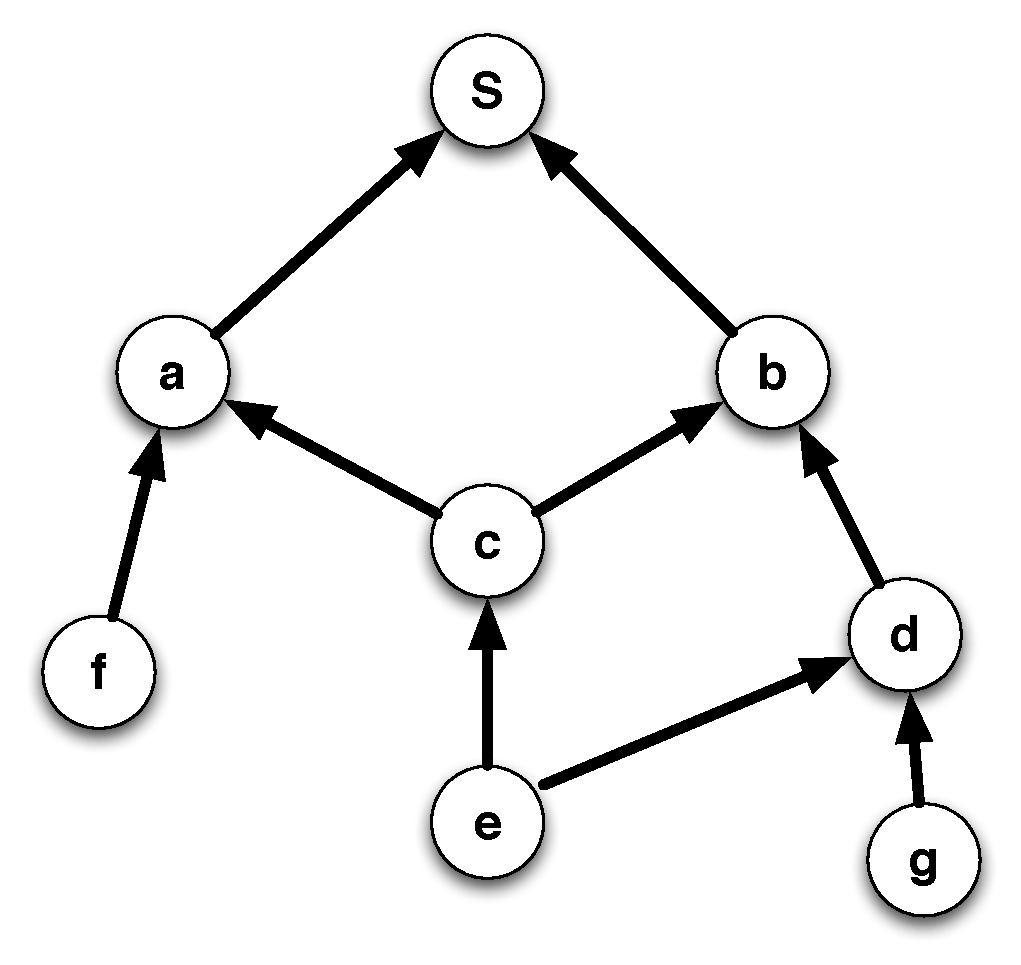
\includegraphics[width=0.3\textwidth]{Figures/Example_1.pdf}
\caption{RPL Basic Construct: DODAGs}
\label{f:dodag}
\end{figure}
%
The DODAG formation thus starts at the DODAG root (initially, the only router which is part of a DODAG), and spreads gradually to cover the whole LLN as DIOs are received, parents and preferred parents are selected and further routers participate in the DODAG. The DODAG root also includes, in DIO messages, a DODAG Configuration Object, describing common configuration attributes for all RPL routers in that network - including their mode of operation, timer characteristics etc. RPL routers in a DODAG include a verbatim copy of the last received DODAG Configuration Object in their DIO messages, permitting also such configuration parameters propagating through the network. \ \\ \ \\
%
A Distance Vector protocol, RPL restricts the ability for a router to change rank. A router can freely assume a smaller rank than previously advertised (i.e. logically move closer to the root) if it discovers a parent advertising a lower rank, and must then disregard all previous parents of higher ranks. The ability for a router to assume a greater rank (i.e. logically move farther from the root) than previously advertised is restricted, to avoid count-to-infinity problems. The root can trigger ``global recalculation" of the DODAG by increasing a sequence number, DODAG version, in DIO messages. \ \\ \ \\
%
The DODAG so constructed is used for installing routes: the ``preferred parent'' of an RPL router can serve as a default route towards the root, or the root can embed in its DIO messages the destination prefixes, included by DIOs generated by RPL routers through the LLN, to which connectivity is provided by the root. Thus, RPL by way of DIO generation provides ``upward routes'' or ``multipoint-to-point routes'' from the sensors inside the LLN and towards the root. \ \\ \ \\
%
``Downward routes'', i.e., the routes from root to sensor nodes, are enabled by having sensors issue Destination Advertisement Object (DAO) messages, propagating as unicast via parents towards the DODAG root. These describe which prefixes belong to, and can be reached via, which RPL router. In a network, all RPL routers must operate in either of storing-mode or non-storing-mode, specified by way of a ``Mode of Operation'' (MOP) flag in the DODAG Configuration Object from the root. Depending on the MOP, DAO messages are forwarded differently towards the root:
%
\begin{itemize}
\item In \textit{non-storing-mode}, an RPL router originates DAO messages, advertising one or more of its parents, and unicast it to the DODAG root. Once the root has received DAOs from an RPL router, and from all routers on the path between it and the root, it can use source routing for reaching advertised destinations inside the LLN.

\item In \textit{storing-mode}, each RPL router on the path between the originator of a DAO and the root records a route to the prefixes advertised in the DAO, as well as the next-hop towards these (the router, from which the DAO was received), then forwards the DAO to its preferred parent.

\end{itemize}
%
``Point-to-point routes'', for communication between devices inside the LLN and where neither of the communicating devices are the DODAG root, are as default supported by having the source sensor transmit via its default route to the DODAG root (i.e., using the upward routes) which will then, depending on the ``Mode of Operation'' for the DODAG, either add a source-route to the received data for reaching the destination sensor (downward routes in non-storing-mode) or simply use hop-by-hop routing (downward routes in storing-mode). In the case of storing-mode, if the source and the destination for a point-to-point communication share a common ancestor other than the DODAG root, a downward route may be available (and used) before reaching the DODAG root. Both of these modes stretch the route by important factors, and lead to significantly longer paths compared to the shortest P2P paths available in the network \cite{nbis2010}. To address this issue, an extension of RPL called RPL-P2P \cite{ietf:rpl-p2p} is currently developed by the IETF. P2P-RPL defines a new mode of operation which provides RPL with a reactive approach to discover better paths on demand between an arbitrary source and destination, without having to go through the root or the first common ancestor of this source and destination.\ \\ \ \\
%
%\subsubsection{RPL Message Emission Timing - Trickle Timers}
%
%\subsubsection{RPL Discussion}
%
While RPL has been specified as \textit{Proposed Standard} in IETF, its applicability and performance in LLNs are not yet fully understood \cite{rpl-observation}. The following lists some limitations and concerns that have emerged concerning basic RPL mechanisms.
%
\paragraph{Requirement of DODAG Root}
%
In RPL, the DODAG Root has both a special responsibility and is subject to special requirements. The DODAG Root is responsible for determining and maintaining the configuration parameters for the DODAG, and for initiating DIO emissions. The DODAG Root is also responsible (in both storing and non-storing mode) for being able to, when downward routes are supported, maintain sufficient topological information to be able to construct routes to all destinations in the network.\ \\ \ \\
%
In a given deployment, selected RPL Routers can be provisioned with the required energy, memory and computational resources so as to serve as DODAG Roots, and be administratively configured as such - with the remainder of the RPL Routers in the network being of typically lesser capacity. In storing mode, the DODAG root needs to keep a routing entry for all RPL Routers in the RPL instance. In non-storing mode, the resource requirements on the DODAG Root are likely much higher than in storing mode, as the DODAG Root needs to store a network graph containing complete routes to all destinations in the RPL instance, in order to calculate the routing table (whereas in storing mode, only the next hop for each destination in the RPL instance needs to be stored, and aggregation may be used to further reduce the resource requirements).
%
\paragraph{Data Traffic Flows}
%
RPL makes a-priori assumptions of data traffic types, and explicitly defines three such traffic types: 
%
\begin{enumerate}
\item sensor-to-root data traffic (multipoint-to-point), which is predominant, 
\item root-to-sensor data traffic (point-to-multipoint), which is rare, and 
\item sensor-to-sensor (point-to-point) data traffic, which is extremely rare.
\end{enumerate} 
%
RPL is suited for networks where sensor-to-root traffic is dominant, by distribution of DIO messages and building of a collection tree. The one way traffic from the sensor to the root can be forwarded through the preferred parent. \ \\ \ \\
%
However, the data traffic characteristics, assumed by RPL, do not represent a universal distribution of traffic types in LLNs. There are scenarios where sensor-to-sensor traffic is a more common occurrence, e.g., in Building Automation scenarios. In addition, there are scenarios, where all traffic is bi-directional. For example, the IETF protocol for use in constrained environments, CoAP \cite{CoAP1,CoAP2}, makes use of acknowledgments to control packet loss and ensure that packets are received by the packet destination. In the four message types defined for CoAP: confirmable, acknowledgement, reset and non-confirmable, the first three are dedicated for sending/acknowledgement cycle.
%
\paragraph{The DAO Mechanisms: Downward and Point-to-Point Routes}
%
In RPL, the ``mode of operation" stipulates that either downward routes are not supported (MOP=0), or that they are supported by way of either storing or non-storing mode. In case downward routes are supported, RPL does not provide any mechanism for discriminating between which routes should or should not be maintained. In particular, in order to calculate routes to a given destination, all intermediaries between the DODAG Root and that destination must themselves be reachable – effectively rendering downward routes in RPL an ``all-or-none" situation. \ \\ \ \\
%
The basic mechanisms in RPL force the choice between requiring all RPL Routers to have sufficient memory to store route entries for all destinations (storing mode)� or suffer increased risk of fragmentation, and thus loss of data packets, while consuming network capacity by way of source routing through the DODAG Root (non-storing mode). \ \\ \ \\
%
In addition, RPL does not explicitly specify how the DAO message are sent, which are used to build ``downward'' routes from root to sensors. This would make the different implementations unlikely to be interoperable. 
%
%\subsection{Simplified Multicast Forwarding (SMF)}
%\label{ss:smf}
%
%Simplified Multicast Forwarding \cite{rfc6621} is developed by IETF, which provides basic IP multicast routing for MANETs. It is mainly applicable in situations where efficient flooding represents an acceptable engineering design trade- off. It consists of two main components: multicast {\em Duplicate Packet Detection} (DPD) and {\em Relay Set Selection} (RSS). 
%
%\paragraph{Duplicate Packet Detection} DPD is used as part of the forwarding process to check if an incoming packet has been previously received (and forwarded) --and therefore should be dropped-- or not. This is achieved, as mentioned in section \ref{ss:flood}, by maintaining a record of recently processed multicast packets, and comparing received multicast packets herewith. A duplicate packet detected is silently dropped and not inserted into the forwarding path of that router, nor delivered to an application.
%
%As proposed by SMF, DPD supports both IPv4 and IPv6 and for each suggests two duplicate packet detection mechanisms: 
%
%\begin{itemize}
%\item  header content identification-based DPD (I-DPD), using packet headers, in combination with flow state, to estimate temporal uniqueness of a packet. 
%\item  hash-based DPD (H-DPD), employing hashing of selected header fields and payload for the same effect.
%\end{itemize} 
%
%\paragraph{Relay Set Selection} RSS is used in SMF to produce a reduced relay set for use when relaying information across the MANET. An efficient reduced relay set is constructed by selecting and  updating, as needed, a subset of all possible routers in a MANET   routing domain to act as SMF forwarders.  Known distributed relay set  selection algorithms have demonstrated the ability to provide and maintain a dynamic connected set for forwarding multicast IP packets. 
%
%SMF supports the use of several relay set algorithms, including ECDS (Essential Connected Dominating Set), S-MPR (Sourcebased Multi-Point Relay), or MPR-CDS. Those algorithms are based on localized election, derived from those explored for efficient topology diffusion in MANET routing protocols.
%
%\subsubsection{Duplicate Packet Detection}
%
%\subsubsection{Relay Set Selection}
